%% This is a sample manuscript marked up using the
%% AASTeX v5.x LaTeX 2e macros.

%% The first piece of markup in an AASTeX v5.x document
%% is the \documentclass command. LaTeX will ignore
%% any data that comes before this command.

%% The command below calls the preprint style
%% which will produce a one-column, single-spaced document.
%% Examples of commands for other substyles follow. Use
%% whichever is most appropriate for your purposes.
%%
%%\documentclass[12pt,preprint]{aastex}

%% manuscript produces a one-column, double-spaced document:

%\documentclass[manuscript]{aastex}

%% preprint2 produces a double-column, single-spaced document:

%% Temporarily commented out.
%%\documentclass[preprint2]{aastex}
%\documentclass[10pt,emulateapj,apj]{emulateapj}
\documentclass{emulateapj}
\usepackage{graphicx}
\usepackage{dcolumn}
\usepackage{bm}
\usepackage{amssymb}
\usepackage{latexsym}
%\documentclass[aps,nofootinbib]{revtex4}
%\usepackage{graphicx}

%% Sometimes a paper's abstract is too long to fit on the
%% title page in preprint2 mode. When that is the case,
%% use the longabstract style option.

%% \documentclass[preprint2,longabstract]{aastex}

%% If you want to create your own macros, you can do so
%% using \newcommand. Your macros should appear before
%% the \begin{document} command.
%%
%% If you are submitting to a journal that translates manuscripts
%% into SGML, you need to follow certain guidelines when preparing
%% your macros. See the AASTeX v5.x Author Guide
%% for information.

%%\newcommand{\vdag}{(v)^\dagger}
\newcommand{\myemail}{robert.speare@gmail.com}

%% If you wish, you may supply running head information, although
%% this information may be modified by the editorial offices.
%% The left head contains a list of authors,
%% usually a maximum of three (otherwise use et al.).  The right
%% head is a modified title of up to roughly 44 characters.
%% Running heads will not print in the manuscript style.

%\shorttitle{AP in gradient vectors}
%\shortauthors{Xiao-Dong Li et al.}

%% This is the end of the preamble.  Indicate the beginning of the
%% paper itself with \begin{document}.

\begin{document}

%% LaTeX will automatically break titles if they run longer than
%% one line. However, you may use \\ to force a line break if
%% you desire.

\title{Applying Alcock-Pacyznski Test to the Gradient Field of Galaxies}

%\author{Robert Speare\altaffilmark{1}, J. Richard Gott\altaffilmark{2}, Juhan Kim\altaffilmark{3}, and
%Changbom Park\altaffilmark{4}}

%\altaffiltext{1}{New York University Abu Dhabi, PO Box 129188, Abu Dhabi, UAE, robert.speare@nyu.edu}
%\altaffiltext{2}{Department of Astrophysical Sciences, Peyton Hall, Princeton University,
% Princeton, NJ 08544-1001, USA}
%\altaffiltext{3}{Center for Advanced Computation, Korea Institute for Advanced Study,
%Heogiro 85, Seoul 130-722, Korea}
%\altaffiltext{4}{School of Physics, Korea Institute for Advanced Study, Heogiro 85, Seoul 130-722, Korea}


%\author{Robert Speare}
%\affil{New York University Abu Dhabi, PO Box 129188, Abu Dhabi, UAE}
%\email{robert.speare@nyu.edu}
%\author{J. Richard Gott}
%\affil{Department of Astrophysical Sciences, Peyton Hall, Princeton University,
% Princeton, NJ 08544-1001, USA}
%\author{Juhan Kim}
%\affil{Center for Advanced Computation, Korea Institute for Advanced Study, 
%Heogiro 85, Seoul 130-722, Korea}
%\email{corresponding author: kjhan@kias.re.kr}

\author{Xiao-Dong Li}
\affiliation{School of Physics, Korea Institute for Advanced Study, 
Heogiro 85, Seoul 130-722, Korea}
\author{Changbom Park}
\affiliation{School of Physics, Korea Institute for Advanced Study, 
Heogiro 85, Seoul 130-722, Korea}
\author{J. E.\ Forero-Romero}
\affiliation{Departamento de F\'{i}sica, Universidad de los Andes, Cra. 1 No. 18A-10, Edificio Ip, Bogot\'a, Colombia}

\begin{abstract}
We propose a model independent measurement of the cosmic expansion history 
by applying the Alock-Paczynski tests to the gradient field of galaxies.
The intrinsically isotropic distributions of the gradient vectors are distorted if we are assuming a wrong cosmology 
to infer the distances of galaxies from their redshifts.
We find the redshift space distortion induced by galaxy peculiar velocities also largely distorts the gradient field,
but can be greatly avoided by looking at the $redshift\ dependence$ of the distortion.
We test the method explicitly on the 27 Horizon Run 3 mock survey data.
Applying the method to 2.4 million physically self-bound halos distributed in the redshift range 0.18-0.6
leads to interesting constraints on $\Omega_m$ and $w$ with 1$\sigma$ errors of $0.07$ and $0.35$.
The slight redshift dependence of the redshift space distortion leads to mild underestimations of 0.5-0.7$\sigma$.
This underestimation can be further corrected by correcting the galaxy redshifts by using perturbation theory,
by skipping 10-30\% high density regions where the galaxy peculiar velocities are large,
by imposing a minimal length cut when estimating the gradient vectors from the nearby region,
and by estimating the redshift space distortion from reference simulations and subtract that.
\end{abstract}

\keywords{large-scale structure of the universe -- cosmology:
numerical}

\newpage 


\section{Introduction}

Cosmic acceleration was discovered in 1998 \citep{Riess1998,Perl1999},
indicating the existence of a new energy component ``dark energy''.
So far the nature of dark energy still remains a mystery.
Without a compelling theoretical explanation of dark energy,
cosmological observations are of essential importance for us.

The well-known Alcock-Paczynski (AP) test \citep{AP1979} is a pure gemoetric probe of the expansion of the Universe
based on the comparison of the observed tangential and radial dimensions of objects 
which are known to be isotropic in the correct choice of cosmology.
So far there have been several methods applying the AP test to the large scale structure.
The most common approach is measuring the anisotropic clustering of galaxies
\citep{Ballinger1996,Matsubara1996}.
This method has been applied in the 2-degree Field Quasar Survey \citep{Outram2004},
the WiggleZ dark energy survey \citep{Blake2011},
the SDSS-II LRG survey \citep{ChuangWang2012},
and the SDSS-III Baryon Oscillation Spectroscopic Survey (BOSS)
\citep{Reid2012,Corredoira2013,Anderson2013}, etc.
The main problem of this method is that,
because the radial distances of the galaxies are inferred from their redshifts,
AP tests are inevitably limited by the peculiar velocities \citep{Ballinger1996},
which causes redshift space distortion (RSD) and leads to apparent anisotropy even if the exact right cosmology is adopted.
This effect should be correctly modeled in the 2-point statistics of galaxy clusterings.

Another interesting idea is measuring the AP distortions by using the symmetry properties of galaxy pairs \citep{Marinoni2010}.
Unfortunately, this method is also limited by the RSD effect.
The distortion of the apparent tilt angles of galaxy pairs due to RSD,
which is found to be dependent on both redshift and cosmological models,
may be rather difficult to be correctly modeled \citep{Jennings2011}.

To avoid the RSD effect, it has also been proposed to use the apparent stretching of voids 
to measure the geometry of the expansion \citep{Ryden1995,LavausWandelt1995}.
This method takes the advantage that the structures in void
regions are much more easily to be modeled compared with high-density regions.
But it also have limitations in that it only utilizes the low density regions of the large scale structure.

In this paper we propose a new method for applying the AP test to the large scale structure of the Universe.
The AP distortion of the cosmic expansion history is encoded in the galaxy distributions.
To measure this distortion, we construct the density field of galaxies and investigating the anisotropies in its gradient field.
An isotropic distribution of gradient vectors indicates that a right cosmology is adopted,
while an anisotropic distribution implies a wrongly assumed cosmology.
This method is similar to the 2-point statistics in that it also focus on the galaxy distributions, but from a different approach.
Moreover, a unique feature of the method is that the high density and low density regions are {\it equally} taken account into the statistics
\footnote{This ``balance'' will is broken when we try to suppress RSD by skipping some high density regions.}.
Methods of 2-point statistics and galaxy pairs pay more attention to the high density regions,
while the void method only focuses on the low density regions.

Like all other proposed methods, it is expected that our method is also affected by RSD,
which distorts the density field in the line of sight (los) direction.
%A successful removal of RSD is of essential importance for the success of the method.
In this work, we find that RSD can be significantly suppressed by focusing on the {\it redshift dependence} of the distortions.
We also proposed four methods to further correct the RSD effect.
We test the method on the Horizon Run 3 (HR3) mock surveys, which are simulated for BOSS.
We find that, by using 2.4 million galaxies in the redshift range 0.18-0.6, 
the method is able to measure $\Omega_m$ and $w$ up to an error of $0.07$ and $0.35$ (1$\sigma$), respectively.

This paper is organized as follows.
In Sec. 2, as a preparation, we perform brief investigations of the AP distortions in different wrong cosmologies.
In Sec. 3 we briefly introduce the data and methodology.
In Sec. 4-6, we apply the method to the mock surveys and assess its performance.
We summarize and conclude in Sec. 7.

\section{Introduction to the Alcock-Pacyznski Test}

Considering something in the Universe which is known to be isotropic.
%We are measuring its tangential size $\Delta r_{\bot}$ and radial size $\Delta r_{\it \parallel}$.
If we happened to know the {\it true} geometry of the Universe, we can correctly measure its radial 
(the direction parallel to the line of sight) 
and tangential (perpendicular to the line of sight) sizes as
\begin{equation}\label{eq:distance}
\Delta r_{\parallel} = \frac{c}{H}\Delta z,\ \ \Delta r_{\bot}=(1+z)D_A(z)\Delta \theta,
\end{equation}
where $H$ is the Hubble parameter, and $D_A$ is the angular diameter distance.
For simplicity let us consider a flat Universe including a matter component with present ratio $\Omega_m$
and a dark energy component with constant equation of state $w$.
Then we have the redshift dependence of the Hubble parameter and the angular diameter distance
\begin{eqnarray}\label{eq:HDA}
 H(z) &=& H_0\sqrt{\Omega_m(1+z)^3+(1-\Omega_m)(1+z)^{3(1+w)}},\nonumber\\ 
 D_A(z) &=& \frac{1}{1+z}r(z)=\frac{1}{1+z}\int_0^z \frac{dz^\prime}{H(z^\prime)}.
\end{eqnarray}
Here $H_0$ is the present value of Hubble parameter,
$r(z)$ is the comoving distance to us.
In the true Universe the tangential and radial sizes of the object are equal to each other, i.e.,
\begin{equation}\label{eq:isotropy}
\Delta r_{\bot}=\Delta r_{\parallel},\ {\rm\ in\ the\ right\ cosmology}.
\end{equation}
In practice, we measure the shape of the object in the redshift space,
adopt a cosmology with assumed value of $\Omega_m$ and $w$, 
and using Eq. (\ref{eq:HDA}) to calculate the spatial sizes of the objects in the tangential and radial directions.
The satisfaction of (or deviation from) Eq. (\ref{eq:isotropy}) enables us to know whether the assumed cosmology is right.
Since we only use the information of isotropy, the intrinsic size of the object does not need to be known.
From Eq. (\ref{eq:distance}) and Eq. (\ref{eq:isotropy}) we find the AP test is sensitive to the quantity
\begin{equation}\label{eq:Fz}
F(z)\equiv\frac{\Delta z}{\Delta \theta}=\frac{(1+z)}{c}D_A(z)H(z).
\end{equation}

\begin{figure}[tpb]
   \centering{
   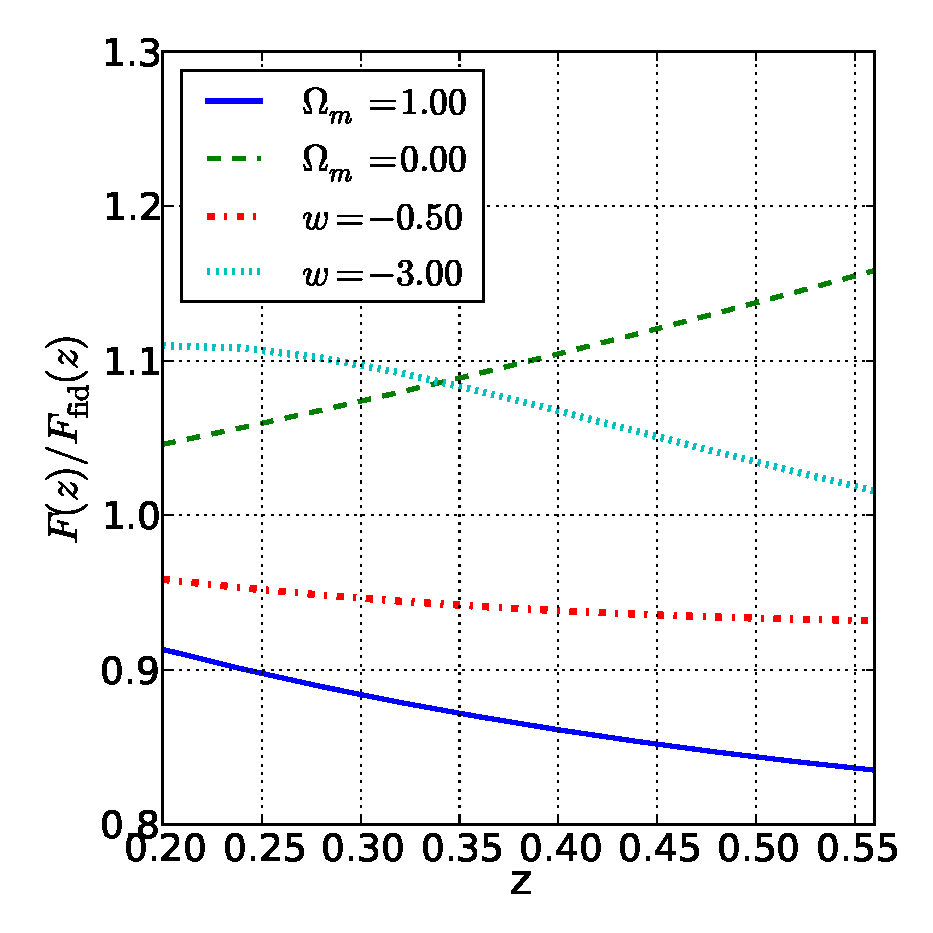
\includegraphics[height=8cm]{ShowStretch.eps}
   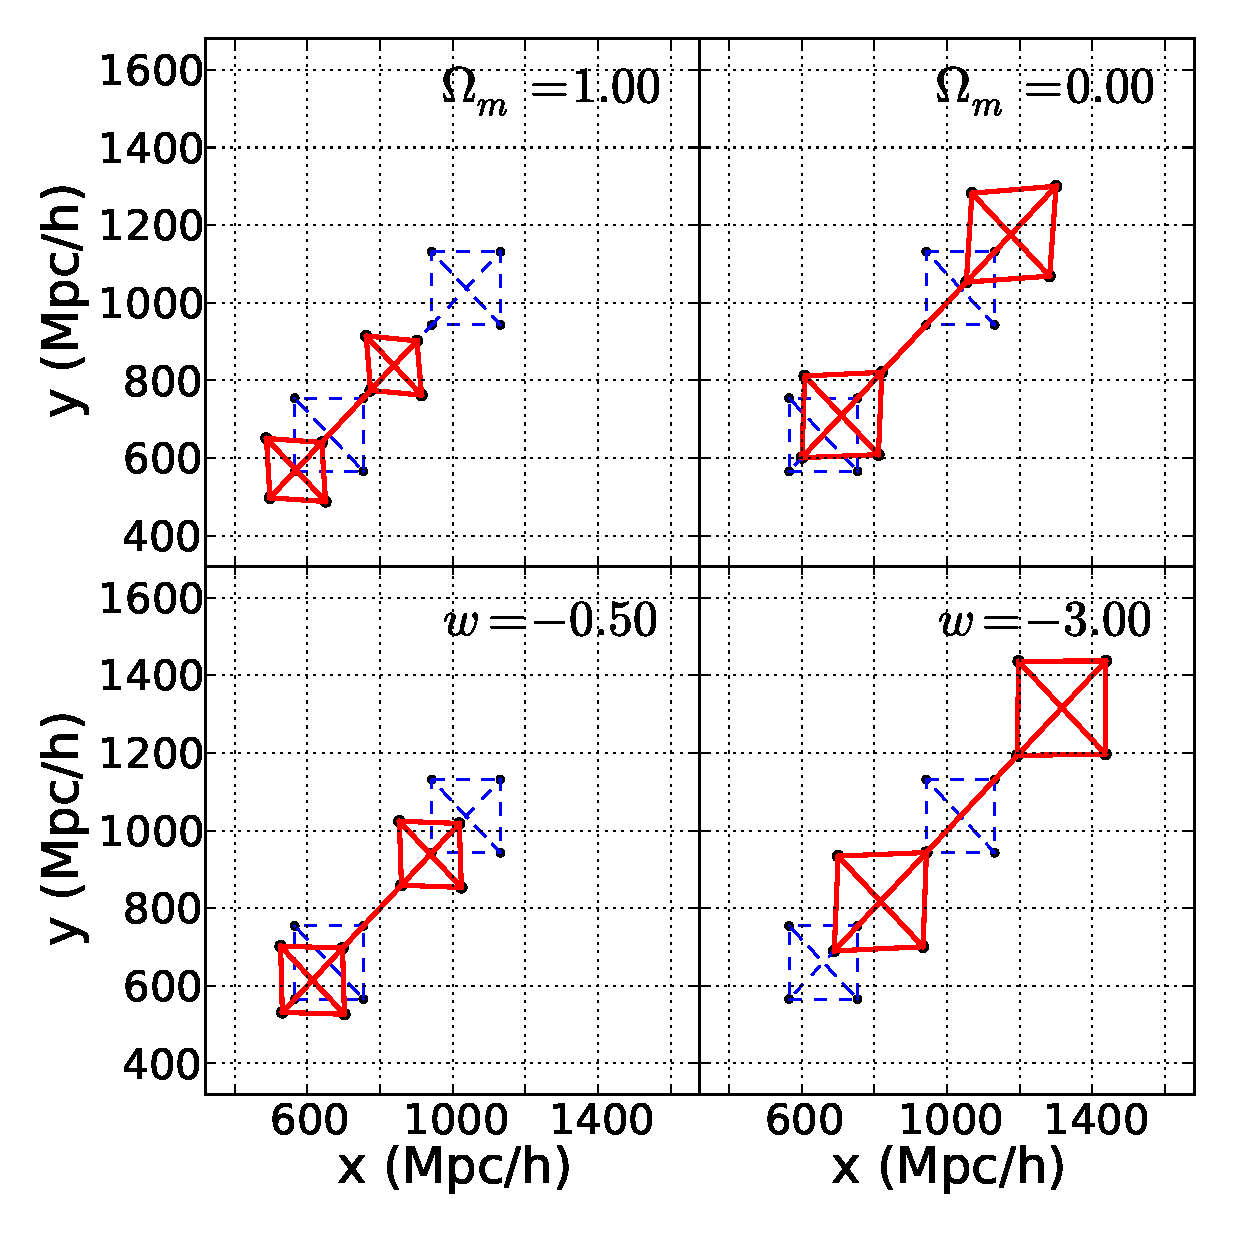
\includegraphics[height=8cm]{ShowAP.eps}}
   \caption{\label{fig_AP} Distortion of isotropy in wrong cosmologies.
   {\it Upper Panel:} Evolutions of $F(z)/F_{\rm fid}(z)$ along with the redshift,
   in the four wrong cosmologies $\Omega_m=1.0$ (blue solid), $\Omega_m=0.0$ (green dashed), 
   $w=-0.5$ (red dot dashed) and $w=-3.0$ (cygan dotted).
   {\it Lower Panel:} The apparent distortions of two perfect squares measured in the four wrong cosmologies (red),
   measured by an observer located at (0,0).
   The shapes and positions of the squares in the right cosmology are also plotted for comparison (blue dashed).}
\end{figure}

An illustration of the AP test is shown in Fig. (\ref{fig_AP})
Assuming that the true Universe is a $\Lambda$CDM model with $\Omega_m=0.26$,
and we are measuring the shape of the object assuming four wrong cosmologies:
$\Omega_m=1.0$ (no dark energy), $\Omega_m=0.0$ (only cosmological constant), 
$w=-0.5$ (quintessence-like dark energy) and $w=-3.0$ (phantom-like dark energy).
%The distortions of isotropy in the wrongly assumed cosmologies are shown in Fig. (\ref{fig_AP}).
The evolutions of functions $F(z)$ (normalized by its value in the right cosmology $F_{\rm fid}(z)$) 
in the wrong cosmologies are shown in the upper figure.
Correspondingly, in the lower figure we show the appeared distortions of two $\approx100 {\rm Mpc/h^2}$ squares in the four wrong cosmologies.
The centers of the squares are located at redshifts 0.33 and 0.55, respectively.
The position of the local observer is located at (0,0).

In the upper figure, we see that the $\Omega_m=1.0$ and $w=-0.5$ cosmologies lead to $F(z) < F_{\rm fid}(z)$.
According to Eq. (\ref{eq:Fz}), this means that the isotropic object appears ``compressed'' along the los direction,
as shown clearly in the upper-left and lower-left panels of the lower figure.
On the contrary, the $\Omega_m=0.0$ and $w=-3.0$ cosmologies have $F(z)<F_{\rm fid}(z)1$, 
meaning that everything appears ``stretched'' along the los.
(see the upper-right and lower-right panels of the right figure).

Moreover, in all plottings we find clear {\it redshift dependence} of distortion.
In the $\Omega_m=1.0$, $\Omega_m=0.0$ and $w=-0.5$ cosmologies, the stretch or compression effect is getting stronger at higher redshift,
while in the $w=-3.0$ cosmology the trend is to the opposite.
As will be discussed in the following context, this phenomenon is of particular importance for our method,
allowing us to measure the cosmological parameters by using the redshift dependence of the anisotropy.

\section{Data and Methodology}

In this paper we test our method by using the Horizon Run 3 (HR3) mock survey data.
The Horizon Runs, provided by the Korean Institute of Advanced Study (KIAS),
provide some of the best raw material for testing our method
\citep{park 2005,horizonrun}. 
The HR3 adopts a standard flat-space $\Lambda$CDM cosmology
with the WMAP5 parameters \citep[]{spergel 2003, komatsu 2011, hinshaw 2013} 
$\Omega_{m}=0.26$, $H_{0}=72{\rm km/s/Mpc}$, $n_{s}=0.96$, etc.
The entire simulation is a cube of 374 billion particles, 
spanning a volume of $(10.815 {~ h^{-1}} {\rm{Gpc}})^3$.
Initial redshift was $z=27$ and $N_{\rm step}=600$ discrete timesteps were taken.

The cold dark matter halos are selected by using the Friend of Friend algorithm
with separation cut off distance 20\% of the mean separation distance. 
To improve cluster identification, HR3 searches for Physically Self Bound (PSB) subhalos 
that are gravitationally self-bound and not tidally disruptable \citep{kim and park 2006}.
This provides a substantial increase in the similarity between simulation and observational data, 
as these dark matter subhalos are sites for LRG formation. 
To simulate the SDSS survey, 
HR3 places 27 observers evenly within its cubical volume and allows each observer to see out to a redshift of $z < 0.7$. 
This creates 27 independent, non-overlapping spherical regions.
The co-moving positions and velocities of all CDM particles are saved as they cross
their past light cone and PSB subhalos are identified from this data. 
In preparation for the SDSS-III LRG catalogue, 
it was assumed that a volume-limited sample would yield a constant number density of $3 \times 10^{-4} (h^{-1}{\rm Mpc})^3$. 
In order to match this prediction, the minimum mass limit of the PSB subhalos was varied with redshift 
and the absolute minimums were set to $9.75 \times 10^{12}~{h^{-1}}{\rm M_{\odot}}$. 
Given these parameters, the physical properties of the HR3 mock surveys match very well with the most recent LRG surveys 
\citep{choi 2010,gott 2009, gott 2008}.

In this work we select out a BOSS-like volume in each mock survey to test the method. 
In each mock survey, we take a hemisphere region with a minimal distance cut $r>500$Mpc/h (corresponding to $z\approx0.18$)
and maximal redshift cut $z=0.6$.
With a constant number density of $3 \times 10^{-4} (h^{-1}{\rm Mpc})^3$ there are $\sim 2.4$ million halos within such a volume.
We embed the whole volume into a $240\times240\times120$ grid
and use the method of smoothed particle hydrodynamics (SPH) to estimate the density and gradient of density at the center of each pixel
\begin{eqnarray}
 &\rho({\bf r}) = \sum_i m_i W({\bf r}-{\bf r}_i,h_{\rm SPH}),\\ 
 &\nabla\rho({\bf r}) = \sum_i m_i \nabla W({\bf r}-{\bf r}_i,h_{\rm SPH}).
\end{eqnarray}
For the smoothing kernel we use the 3rd order B-spline functions,
which has non-zero value in a sphere with radius 
\begin{equation}
r_{\rm SPH}=2\times h_{\rm SPH}\ {\rm Mpc/h}. 
\end{equation}
%In our coordinate the observer was located at the point (0,0,0),
%the ranges of $x$ and $y$ are from -1570 to 1570 Mpc/h, 
%while the range of $z$ is from 0 to 1570 Mpc/h.

\section{The Effects of AP and RSD on the Gradient Field}

In this section we investigate how the isotropic gradient field is distorted by AP or RSD.
For statistical quantity, we use the $\cos$ of the angle between the gradient vector and the radial direction
\begin{equation}
 \mu\equiv |\cos \theta|,\ \theta\equiv \frac{{\bf r}\cdot\nabla\rho({\bf r})}{|{\bf r}|\times|\nabla\rho({\bf r})|}.
\end{equation}
For an isotropic density field with homogeneous distribution of directions of the gradient vectors,
we expect $\mu$ uniformly distributed in (0,1).
We find it is useful to look the mean value
\begin{equation}
 \langle\mu\rangle \equiv {\sum_{i=1,... n} \mu_i}/n,
\end{equation}
where $n$ is the number of gradient vectors sampled in the whole filed.
For an isotropic filed we expect $\langle\mu\rangle=0.5$.

\subsection{AP Effects on the Gradient Field}

\begin{figure*}[tpb]
   \centering{
   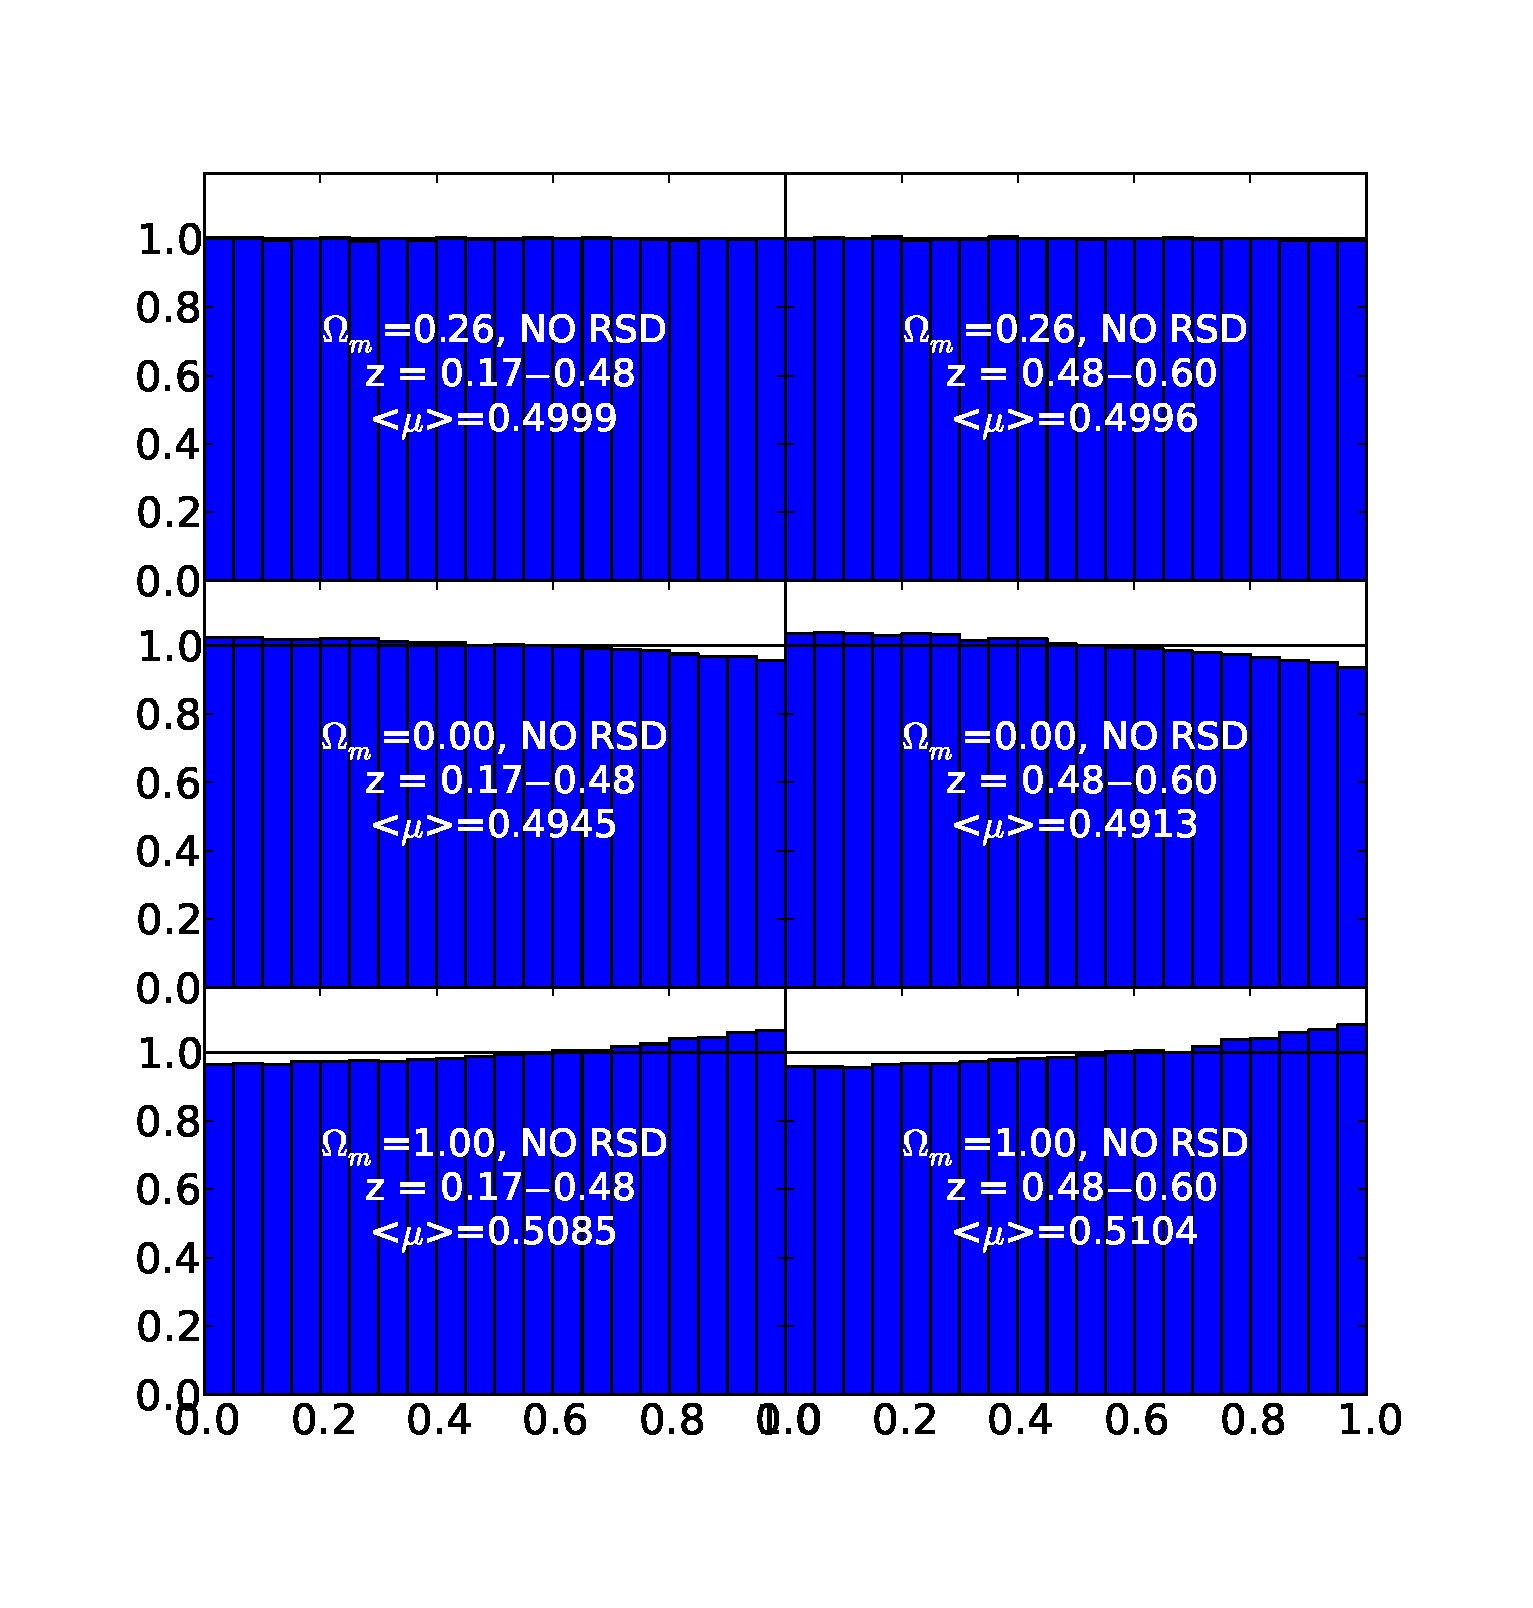
\includegraphics[height=9.2cm]{mu_NORSD.eps}
   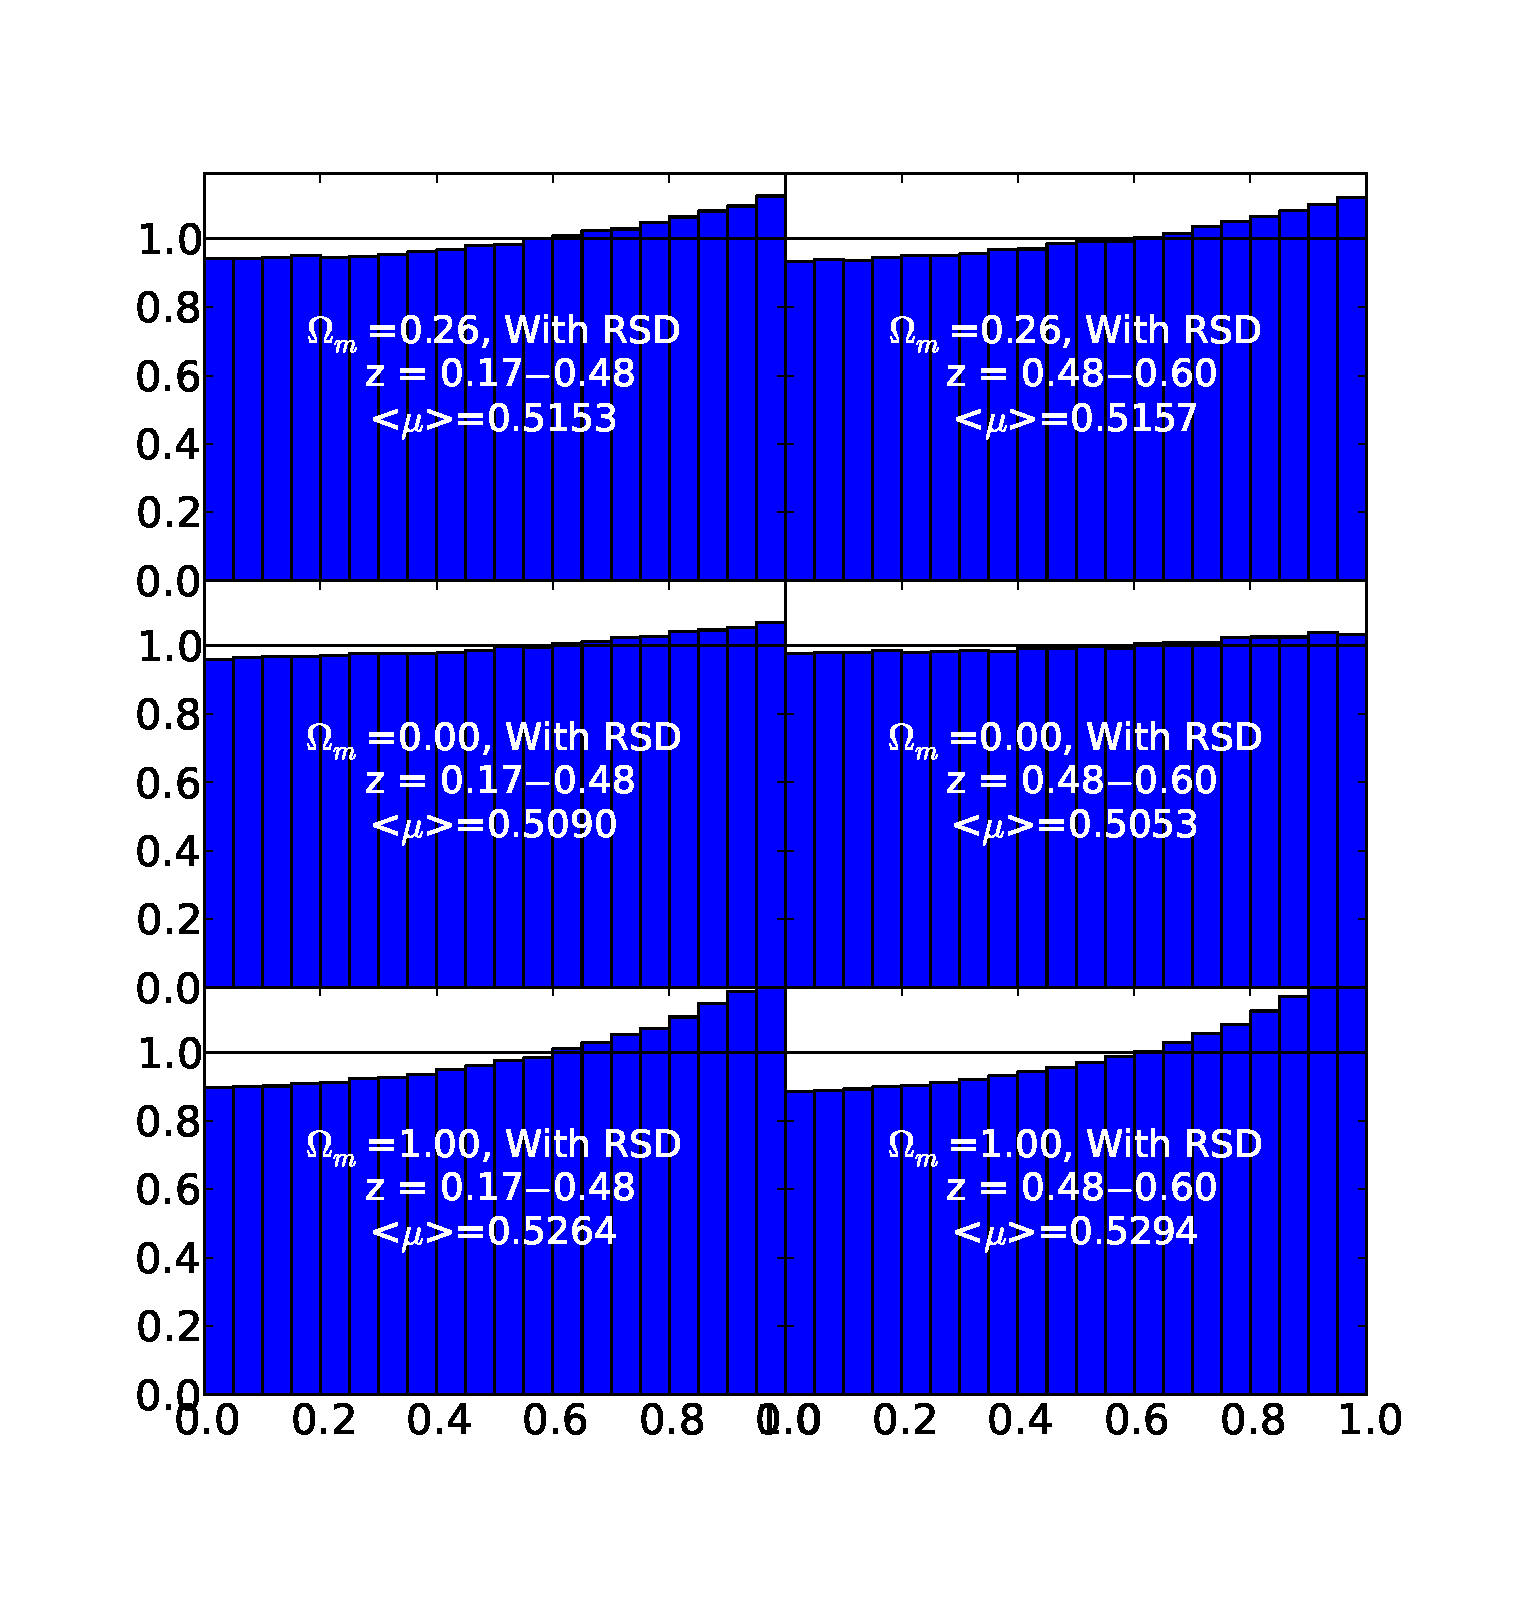
\includegraphics[height=9.2cm]{mu_WithRSD.eps}}
   \caption{\label{fig_muhists} Histograms of $\mu=|\cos\theta|$ measured from the gradient fields, 
   in cases of no RSD (left panel) and with RSD (right panel). 
   From top to bottom, we show the results when assuming a cosmologies with $\Omega_m$ = 0.26, 0 and 1.
   To see the redshift dependence of the distortion, 
   we show results of the low redshift region ($z<0.48$) and high redshift region ($z>0.48$), respectively.
   The distortion of the isotropy due to RSD is more sever than the AP distortion,
   but the redshift dependence of RSD distortion is much smaller than the redshift dependence of AP distortion.}
\end{figure*}

In this section we investigate AP effects on the gradient field.
Without loss of generality, we adopt three cosmologies, 
the right cosmology $\Omega_m=0.26$, the Standard CDM (SCDM) cosmology $\Omega_m=1.0$,
and the extreme case of the dark energy dominate cosmology $\Omega_m=0.0$.
In all cosmologies we fix $w=-1$.
The histograms of $\mu$ measured in the gradient fields constructed assuming the three cosmologies are plotted in Fig. \ref{fig_muhists}.
To show the {\it redshift dependence of the AP distortion}, 
we present the histograms in the redshift ranges of $z<0.48$ and $z>0.48$, respectively.
The left figures show the results without considering RSD, 
and the right figures show the with RSD results.

As expected, in the right cosmology we get uniform distributed $\mu$s (the first row of Fig. \ref{fig_muhists}),
with mean value $\langle\mu\rangle$ rather close to 0.5.
The small discrepancy is due to the statistic error (which is about $4\times10^{-4}$).
In the SCDM cosmology, since structures are compressed along the los,
the radial component of gradient vectors are amplified, 
and we expect an enhanced distribution of $\mu$ at large values.
Our expectation is confirmed by the histogram shown in the last row of Fig. \ref{fig_muhists},
where $\langle\mu\rangle>0.5$ is detected at 40$\sigma$ confidence level (CL).
For the $\Omega_m=0.0$ cosmology, the situation is the opposite and we find $\langle\mu\rangle<0.5$ as expected, 
detected at about 60$\sigma$ CL.

By comparing the low redshift and high redshift histograms,
we also find clear redshift dependence of the AP distortion in the gradient fields.
For the $\Omega_m=0.0$ cosmology, 
we find $\langle\mu\rangle=0.4945$, 0.4913 for $z<0.48$ and $z>0.48$,
both below 0.5 but the $z>0.48$ part is smaller.
The difference between the mean values $\langle\mu\rangle$ of the two parts is
 $\langle\mu(z>0.48)\rangle\ -\ \langle\mu(z<0.48)\rangle= -0.0032$, 
which is a 10$\sigma$ CL signal considered the statistic fluctuation.
Similarly, for the $\Omega_m=1.0$ case we find a difference of $0.0019$, a 5$\sigma$ CL detection.
Compared with the deviation from $\langle\mu\rangle=0.5$ (40-60$\sigma$),
the deviation from no redshift dependence is detected at much lower level (5-10$\sigma$),
but still much larger than the statistic fluctuation.

\subsection{RSD Effects on the Gradient Field}

To assess the influence of RSD on the gradient field,
in this subsection we present the results when the RSD effect is included in the gradient field.

The with RSD histograms of $\mu$ in the three cosmologies are plotted in the right figure of Fig. \ref{fig_muhists}.
Unfortunately, we find RSD has a rather large effect on the gradient field.
RSD distorts the structure along the los, amplifies the radial component of $\mu$,
leading to an apparent anisotropy similar to the result of a large $\Omega_m$ cosmology.
As a result, in the right cosmology we get $\langle\mu\rangle=0.5155$.
The deviation from uniform is at nearly 100$\sigma$ CL, 
even much larger than the $\Omega_m=1.0$ cosmology.
Due to RSD, the three cosmologies all yield to $\langle\mu\rangle>0.5$.
So it becomes impossible to know the correct value of $\Omega_m$ by checking the deviation of $\langle\mu\rangle$ from 0.5.

Despite the large effect of RSD on $\langle\mu\rangle$, however, 
we find the redshift dependence of $\langle\mu\rangle$ is not much affected by RSD.
In the right cosmology, although the uniform distribution seriously destroyed by RSD,
the difference between the nearby and farther parts $\langle\mu(z>0.48)\rangle\ -\ \langle\mu(z<0.48)\rangle= 0.0004$,
which is of the same order of the statistical fluctuation.
Correspondingly, in the $\Omega_m=1.0$ and $\Omega_m=0.0$ cosmologies the difference are -0.0037 and 0.003,
which are close to the corresponding no RSD results -0.0032 and 0.0019.
As a result, we are still able to distinguish the wrong cosmologies from the right one
by looking at the redshift dependence of $\langle\mu\rangle$.

In all we conclude that {\it RSD effect is large but its redshift dependence is small}.
The redshift dependence of $\langle\mu\rangle$ is suitable for cosmological analysis.
Notice that it still suffers from the slight redshift dependence due to RSD.
In the right cosmology, there is a positive difference $0.0004$ introduced by RSD, 
which can be compensated by a slightly smaller $\Omega_m$.
As a result, we are expected to have an underestimate of about 0.03 in $\Omega_m$
\footnote{For $\Omega_m = 0$ we have $\langle\mu(z>0.48)\rangle\ -\ \langle\mu(z<0.48)\rangle= 0.0037$, 
so a difference of $0.0004$ roughly corresponds to $0.0004\times\frac{0.26}{0.0037}\approx0.03$.}.

Based on the above analysis, we construct the following likelihood function to probe cosmological parameters
\begin{equation}\label{eq:like}
 \mathcal{L}\propto e^{-\chi^2/2},\ \ \chi^2\equiv \left(\frac{\langle\mu\rangle(z<z_{\rm mid})-\langle\mu\rangle(z>z_{\rm mid})}
 {\sqrt{{\sigma}_{\langle\mu\rangle(z<z_{\rm mid})}^2+{\sigma}_{\langle\mu\rangle(z>z_{\rm mid})}^2}}\right)^2.
\end{equation}
where $z_{\rm mid}$ is the middle redshift which split the volume into two equal volume parts.
A wrong cosmology leads to a redshift dependence in the anisotropy,
resulting a large $\chi^2$ and is thus disfavored.
In this work, we only consider the cosmologies with either wrongly assumed $\Omega_m$ or wrongly assumed $w$,
and we find that comparing the $\langle\mu\rangle$ in two volumes at different redshifts seems to be good enough.
In more complicate case (i.e., more cosmological parameters, dynamical dark energy), 
it may be helpful to generalize Eq. \label{eq:like} and made a comparison among 3 or more volumes at different redshifts.

\section{Correcting the Redshift Dependence of RSD}

In the previous section we show that the by focusing on the redshift dependence of the gradient field we can avoid RSD to a large extent,
but the $\Omega_m$ is still mildly underestimated due to the redshift dependence of RSD distortion.
In this paper, we consider four possible ways to further correct this error.
In this section, we introduce the basic concepts of these methods, commenting their advantages an disadvantages.
The performance assessment of these methods will be presented in the next section.

\subsection{Correcting Galaxy Redshifts from Perturbation Theory}
 
From the distribution of galaxies we can estimate the peculiar velocity of each galaxy from the perturbation theory.
The simplest estimation is from the linear regime result
\begin{equation}
  {\bf{v}}\left( {\bf{r}} \right) =
\frac{Hf}{4\pi }\int d^3 {\bf{r}}^{\prime
} \delta_{m}\left( \mathbf{r}^{\prime }\right) \frac{\left( \mathbf{r}^{\prime
}-\mathbf{r}\right) }{\left| \mathbf{r}^{\prime }-\mathbf{r}\right| ^3}.
\label{peculiar}
\end{equation}
Here ${\bf v}\left( {\bf{r}} \right)$ is the peculiar velocity of a galaxy with comoving coordinate $\bf r$,
$f$ is the growth factor, 
and the density contrast is $\delta_{m}\equiv (\rho_m-\bar{\rho}_m)/\bar{\rho}_m$,
where $\bar{\rho}_m$ is the average density.
In real observational cases the right hand side of Eq. (\ref{peculiar})
is usually divided by a bias factor $b$ since galaxies are biased tracers of dark matter.

\begin{figure}[tpb]
   \centering{
   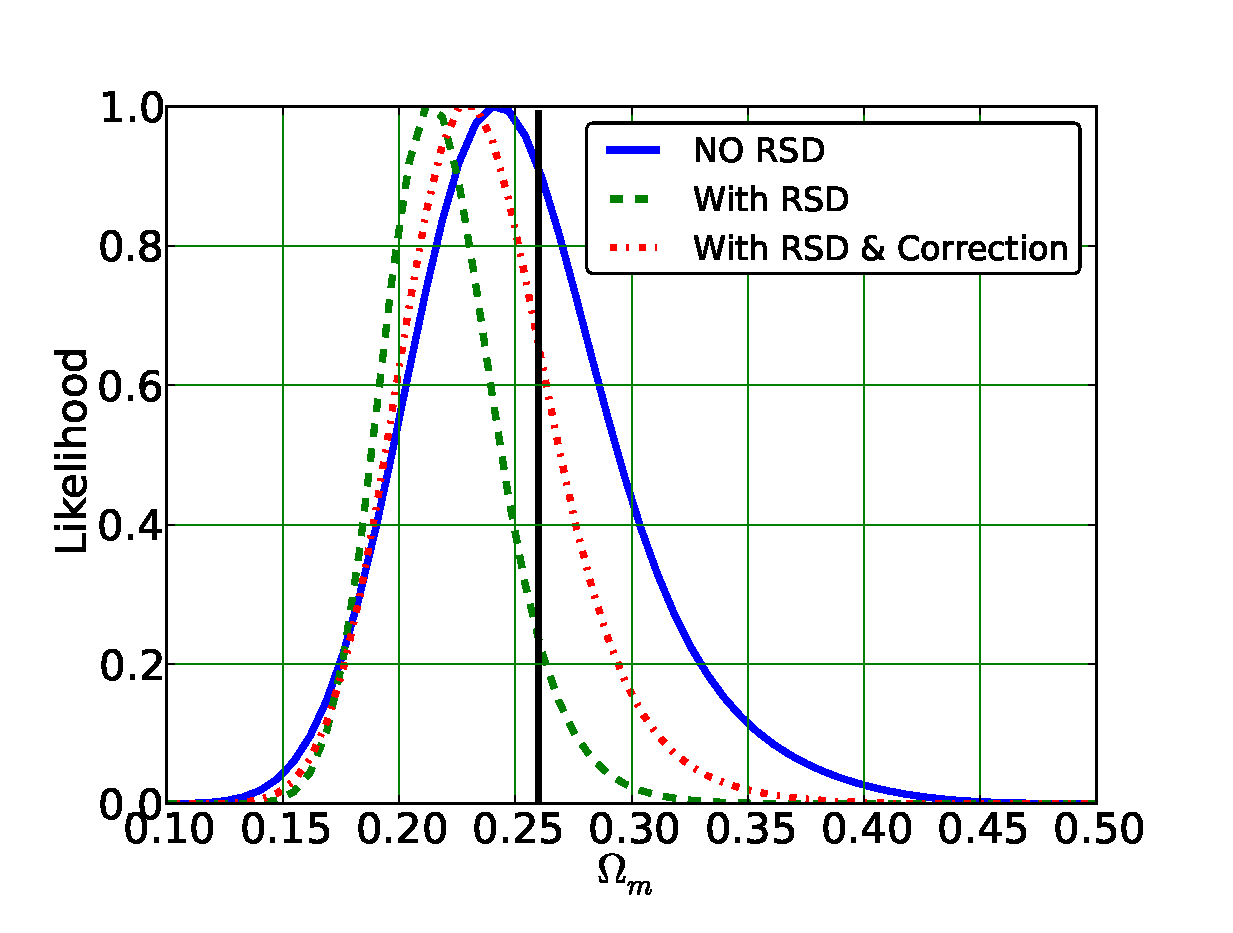
\includegraphics[height=6cm]{1Like.eps}}
   \caption{ \label{fig_1like} Likelihood curve of $\Omega_m$ from one of the 27 mock surveys.
   If there is no RSD effect (blue solid), the method yields to right estimation of $\Omega_m$.
   Considering RSD effect (green dashed) the estimated $\Omega_m$ is mildly underestimated.
   When we correct the redshifts of galaxy by using the velocity estimated from Eq. \ref{peculiar},
   this underestimation is partly corrected (red dotted).
   Notice that this figure shows a high quality sample from the 27 constriants and in most cases the performance is not so good.}
\end{figure}

In this work we try Eq. (\ref{peculiar}) to correct the distorted positions of galaxies.
As an example, Fig. \ref{fig_1like} shows the likelihood curves of $\Omega_m$ reconstructed from one of the 27 mock data.
Our method yields a good estimation $\Omega_m\approx0.25$ when ignoring the RSD effect on the gradient field
\footnote{Using the real redshifts (not distorted by RSD) of galaxies to infer their distances and construct the gradient field.
In the following we will mention this as ``no RSD''. 
The result when considering RSD effect will be mentioned as ``with RSD''.}.
Considering RSD distortions in the galaxy positions leads to an underestimated constraint $\Omega_m\approx0.21$.
Correcting the RSD distortions by using linear perturbation theory mildly corrects the result to $\Omega_m\approx0.225$.

Notice that Fig. \ref{fig_1like} is a high quality example and in most cases the perturbation theory does not give good result.
%Unfortunately, we find it does not lead to evident improvement of the result.
The reason is that Eq. (\ref{peculiar}) only accounts for the linear order Kaiser effect.
The non-linear Figure of God effect, which may have more significant influence on the gradient vectors, is not corrected.
Besides, the precision of the $\rho_m$, which is estimated from the halos with mean separation $15$ Mpc/h, 
is also limited by the sparseness of the sample. This further limits the ability of the method.

 
\subsection{Applying Minimal Length Cut in SPH}
 
The peculiar velocity effect can be suppressed by imposing a {\it minimal} length cut $r_{min}$ 
when we use the SPH technique to estimate the gradient vectors, i.e., 
\begin{equation}
 \nabla\rho({\bf r}) = \sum_{|{\bf r}-{\bf r}_i|>r_{min}}
 m_i \nabla W({\bf r}-{\bf r}_i,h).
\end{equation}
Distortions of the positions of very nearby galaxies can lead to
significant changes in the direction of ${\bf r}-{\bf r}_i$, 
resulting large errors in the estimated direction of the gradient vector.
As will be discussed in the next subsection,
for the HR3 mock survey data we find taking a cut $r_{min}\approx15$ Mpc/h can lead to a visible suppression of the RSD effect.
 
\subsection{Skipping High Density Regions}

Galaxies in the high density regions possess large peculiar velocities.
So skipping some high density region shall be helpful to improve the statistics.

\begin{figure}[tpb]
   \centering{
   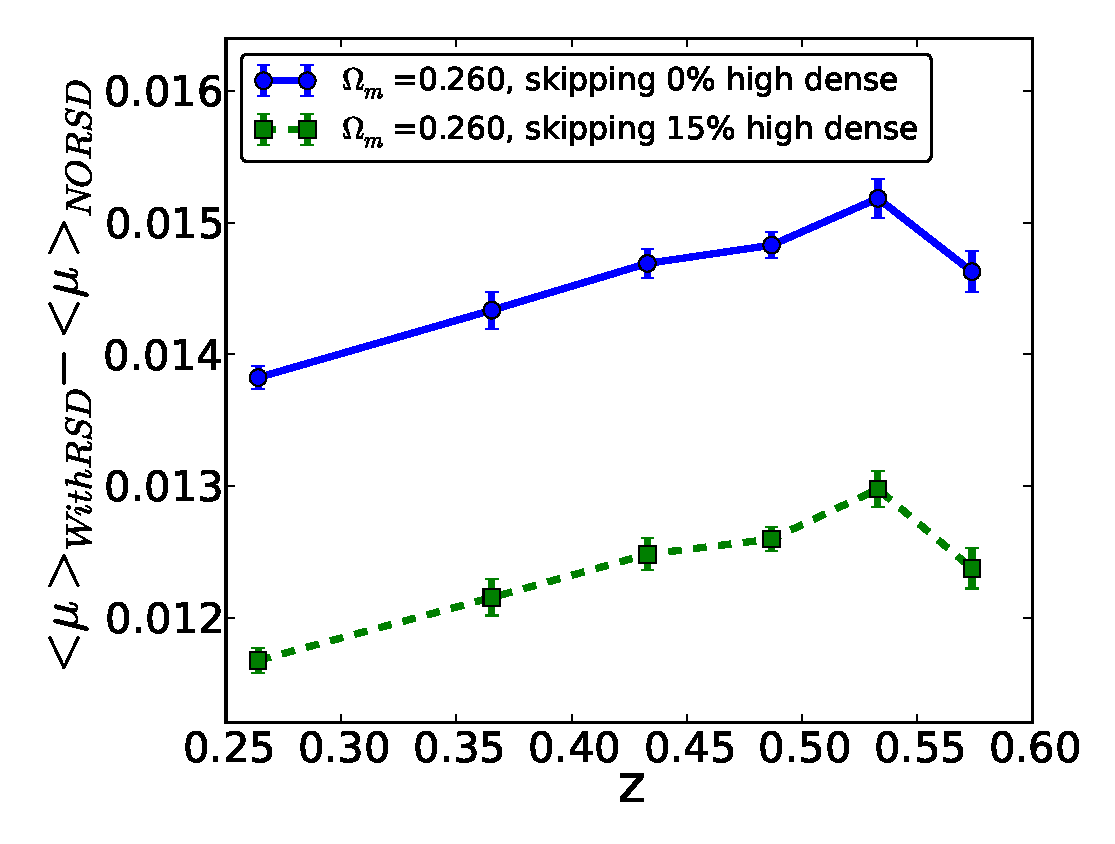
\includegraphics[height=6cm]{mu_z.eps}}
   \caption{ \label{fig_mu_z} Redshift dependence of $\langle\mu\rangle$ due to RSD.
   The evolution of $\langle\mu\rangle_{\rm With\ RSD}-\langle\mu\rangle_{\rm No\ RSD}$ along with redshift is plotted.
   The blue solid curve shows the result from the whole gradient field.
   The green green curve shows the result when we drop $\approx15\%$ high density regions.
   Skipping high density regions suppress RSD effect, but does not suppress its redshift dependence too much.}
\end{figure}

We test the idea on the mock data.
Fig. \ref{fig_mu_z} shows {\it the redshift dependence of $\langle\mu\rangle$ due to RSD},
where we calculate the $\langle\mu\rangle$ of the no RSD and with RSD gradient fields (in the right cosmology),
and plot the difference between the no RSD and with RSD, result 
($\langle\mu\rangle_{\rm With\ RSD}-\langle\mu\rangle_{\rm No\ RSD}$) in the redshift range $z=0.2-0.6$.
The differences when considering the whole gradient field and skipping $\approx15\%$ high density regions are shown for comparison
\footnote{We show the averaged results from 27 mock surveys. 
The gradient fields are reconstructed from mass density field with a smoothing length $12.5$ Mpc/h 
(or equivalently $r_{\rm SPH}=0-25$ Mpc/h).
The result can be slightly different if we use the the number density field or change the smoothing length.}.
We find that skipping high density region can evidently suppress the RSD effect on $\langle\mu\rangle$.
By skipping 15\% high density regions,
the amplitude of the $\langle\mu\rangle_{WithRSD}-\langle\mu\rangle_{NORSD}$ is suppressed by $\approx15\%$.
However, the redshift dependence of the $\langle\mu\rangle$ due to RSD is almost unaffected.
To see this let's compare the maximal and minimal values in the two curves, 
located at $z\approx0.26$ and $z\approx0.53$.
The no skipping result shows a difference of 0.00136 between the two redshifts, 
while the $\%15$ skipping result shows a difference of 0.00130, which is only 4.5\% smaller.
So the performance of this method is limited since we are using the deviation from no redshift dependence of the $\langle\mu\rangle$
(rather than the deviation from $\langle\mu\rangle$=0.5) to probe AP.
 
\subsection{Estimating RSD Effect from Reference Simulations}
\label{sec_corec_ref_sim}

\begin{figure*}[tpb]
   \centering{
   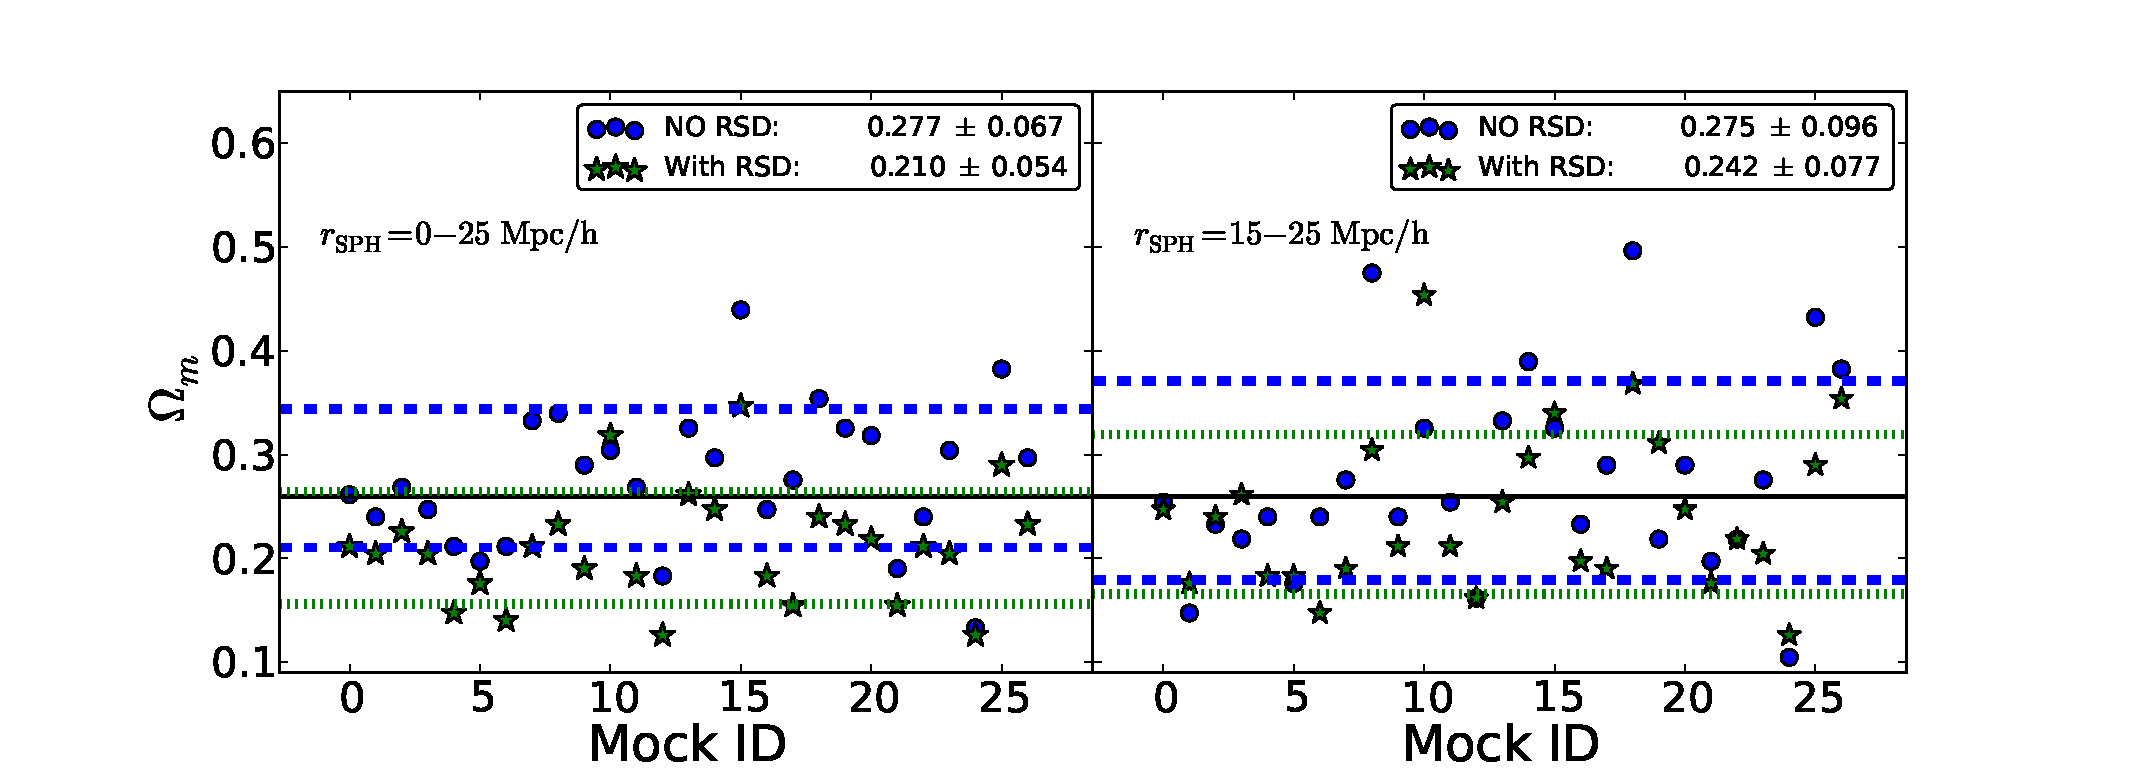
\includegraphics[scale=0.4]{multLikes.eps}
   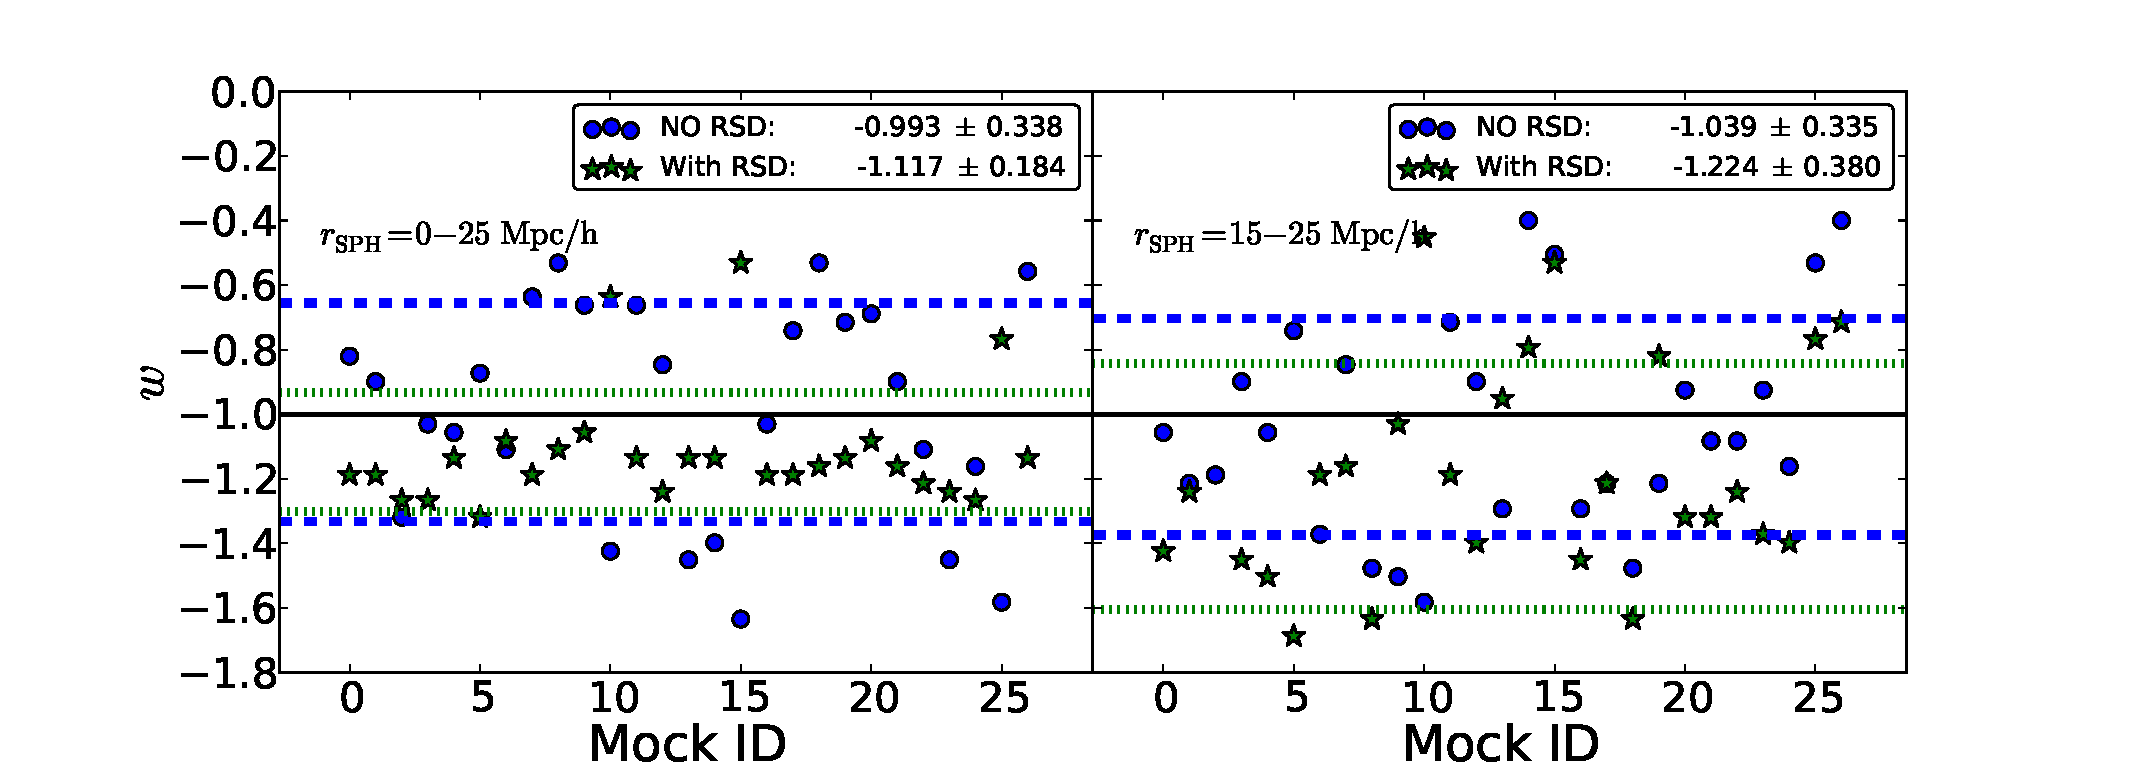
\includegraphics[scale=0.4]{multLikes_w.eps}}
   \caption{ \label{fig_multlike} Conditional constraints on $\Omega_m$ (upper panels) and $w$ (lower panels) from the 27 mock surveys.
   The left panels show the results with a smoothing length $12.5$ Mpc/h.
   The right panels show the results when we further impose a minimal distance cut $15$ Mpc/h in the SPH.
   No RSD and with RSD best-fits of 27 mock surveys are shown in blue circles and green stars.
   After averaging the 27 results, the obtained best-fits and 1$\sigma$ uncertainties of the no RSD and with RSD cases 
   are marked by blue dashed and green dotted lines (the values are presented in the legends).
   Our fiducial cosmology $\Omega_m$=0.26, $w=-1$ is marked by the horizontal black lines.
   In all panels, no RSD results are in excellent agreement with the fiducial cosmology.
   Considering RSD effect in the gradient field yields to acceptable $\approx0.5-0.7\sigma$ underestimations.
   The underestimation is partially corrected if we impose a minimal distance cut when calculating the gradient vectors 
   by using the SPH technique, in the cost of increased error bars due to the loss of the information.}
\end{figure*}

An ultimate method for correcting RSD is to estimate the redshift dependence of $\langle\mu\rangle$ from reference simulations 
(e.g., Fig. \ref{fig_mu_z}) and subtract that from $\langle\mu\rangle(z)$.
We applied this to our mock data and find the RSD effect is, as expected, almost completely removed.
While this method certainly works perfectly when we use the result from simulation to correct itself, 
when applying to real observational data it suffers from two problems:
\begin{itemize}
 \item The discrepancy between the fiducial cosmology assumed in the simulation and the true Universe.
 This error can be corrected by several ways:
 choosing a set of parameters close enough to the real cosmology;
 adopting an iterative algorithm (run the simulations with some assumed parameters 
 $\rightarrow$ estimate cosmological parameters from observations, adopting the RSD correction based on simulation
 $\rightarrow$ rerun the simulations by using the estimated cosmological parameters and repeat the above procedure until convergence);
 run a series of simulations to cover a large enough space of parameters; etc.
 \item Lack of fidelity of the simulation in describing the position and velocities distributions of the galaxies.
 To avoid this problem one needs a high quality simulation faithful to the real observation. 
\end{itemize}
Discussion of the above issues is beyond the scope of this work.
It is important to address these issues when applying the method to real observational data.

\section{Performance Assessment from the 27 HR3 Mock Surveys}

We test the method on the 27 HR3 mock survey data.
This allows us assess both the statistical errors and cosmic variance in the result.
The results are shown in Fig. (\ref{fig_multlike}).
Upper panels show the constraints on $\Omega_m$ (with fixed $w=-1$),
while lower panels show the constraints on $w$ (with fixed $\Omega_m = 0.26$).
In all results we apply a smoothing length $h_{SPH}=12.5$ Mpc/h.
The two right panels show the result when a minimal length cut $15$ Mpc/h is imposed to suppress RSD ($r_{SPH}=15-25$ Mpc/h).
More results, including the constraint on $\Omega_m$ when we impose the RSD correction from the perturbation theory, 
the minimal length cut, dropping high density regions, and the RSD correction by using reference simulations, 
are presented in Table \ref{Table1}.

The upper-left and lower-left panels shows the no RSD constraints of $\Omega_m$ and $w$.
Averaging over the 27 mocks, we get a constraint $\Omega_m=0.277\pm0.067$ and $w=-0.993\pm0.338$,
in good consistent with the fiducial values.
Considering RSD the constraints become $\Omega_m=0.210\pm0.054$ and $w=-1.039\pm0.335$,
with an underestimation of 0.7$\sigma$ and 0.5$\sigma$, respectively.
Notice that the error bars of $\Omega_m$ are evidently larger than the ones in Fig. (\ref{fig_1like}),
which are only statistical errors.
This manifests the effect of cosmic variance
\footnote{Due to the limited volume of the survey, 
the gradient field can have some intrinsic redshift dependence even the correct cosmology is taken.}.

While an underestimation of less than 1$\sigma$ is acceptable,
it is always better to find a way correcting that.
The right panels show the results when imposing a minimal distance $r_{min}=15$ Mpc/h in the SPH to suppress RSD.
We get $\Omega_m=0.242\pm0.077$ and $w=-1.224\pm0.380$, which are in better consistent with the fiducial model.
The cost is that the error bars are amplified due to the loss of information in the distance cut.

\begin{table}
\begin{center}
\caption{Constraints on $\Omega_m$ after applying different various RSD correction methods. }
\begin{tabular}{|c|c|c|}
\hline
RSD Correction Method       ~&~No RSD      ~&~With RSD \\
\hline
No Correction        ~&~$0.277\pm0.067$ ~&~$0.210\pm0.054$    \\
\hline
Imposing $r_{min}=15$ Mpc/h~&~$0.275\pm0.096$ ~&~$0.242\pm0.077$ \\
\hline
Linear Perturbation Theory ~&~ -  ~&~ $0.208\pm0.055$ \\
\hline
Skipping 10\% High Density ~&~ 0.273$\pm$0.059 ~&~  0.216$\pm$0.051 \\
\hline
Skipping 20\% High Density ~&~ 0.271$\pm$0.060 ~&~  0.218$\pm$0.051 \\
\hline
Skipping 30\% High Density ~&~ 0.267$\pm$0.060 ~&~  0.220$\pm$0.056 \\
\hline
Skipping 40\% High Density ~&~ 0.267$\pm$0.067 ~&~  0.219$\pm$0.060 \\
\hline
Skipping 50\% High Density ~&~ 0.264$\pm$0.072 ~&~  0.218$\pm$0.063 \\
\hline
Estimating RSD from Simulation  ~&~ - ~&~  0.275$\pm$0.074 \\
\hline
\end{tabular}\label{Table1}
\end{center}
\end{table}

Except imposing a minimal distance cuts in SPH, we also have three other methods to correct RSD, i.e.,
correcting galaxy redshifts by using perturbation theory,
skipping high density regions, 
and correcting RSD by estimating it from reference simulation.
The constraints on $\Omega_m$ after applying these methods are shown in Table \ref{Table1}.
We briefly introduces them as follows.

After correcting RSD based on linear perturbation theory, 
the constraints on $\Omega_m$ becomes $0.208\pm0.055$ (no length cut) and $0.253\pm0.090$ 
(with length cut 15 Mpc/h; not shown in the Table).
Compared with the no correction results they are not great improvements.
On the other hand, the error bars are amplified due to errors introduced in the correction procedure.

Suppressing RSD by skipping high density regions leads to slightly suppression of RSD.
The with RSD constraint $\Omega_m=0.210\pm0.054$ becomes $0.216\pm0.051$,
$0.218\pm0.051$, $0.220\pm0.056$, $0.219\pm0.060$ and 0.218$\pm$0.063 
after we skipping 10\%, 20\%, 30\%, 40\% and 50\% high density regions.
It seems that skipping 10\%-30\% can lead to slight suppression of RSD.
Skipping more regions cannot further suppress RSD but increases the error bar.

Modeling the RSD effect on $\langle\mu\rangle$ (Fig. \ref{fig_mu_z}) and subtract that from the obtained $\langle\mu\rangle$,
we get $\Omega_m=0.275\pm0.074$, which is in excellent agreement with the no RSD constraint 0.277$\pm$0.067,
meaning that RSD is almost completely removed.
This is of course expected since we are using the results from the simulations to correct themselves.
But for real observational data the estimation may be biased due to reasons mentioned in Sec. \ref{sec_corec_ref_sim}.

Finally, we mention that all the results above are obtained by using the mass density field of galaxies.
Using the number density field yield to similar results for all methods except the linear perturbation method,
where the larger errors in the estimated peculiar velocities make the method perform worse.

\section{Concluding Remarks}

As a summary, we propose a new method for applying the AP tests to the gradient fields of galaxies.
The intrinsically isotropic distributions of the gradient vectors are distorted if we assume a wrong cosmology 
to infer distances of galaxies from redshifts.
We find the RSD effect can be greatly suppressed by focusing on the redshift dependence of the distortion.

The method is tested explicitly on the 27 HR3 mock survey data,
for each of them we select out a BOSS-like volume,
with 2.4 million halos uniformly distributed in the redshift range 0.18-0.6.
We find the method leads to interesting constraints on $\Omega_m$ and $w$ with error bars of $0.07$ and $0.35$.
The redshift dependence of RSD leads to acceptable underestimations of $0.5-0.7\sigma$.

We consider four methods to further correct the redshift dependence of the RSD distortion.
Correcting RSD from linear perturbation theory does not lead to evident improvement of the result,
since it does not corrects the Figure of God effect, and is limited by the sparseness of our sample.
By imposing a minimal length cut 15 Mpc/h in SPH, 
we correct the constraint on $\Omega_m$ from $0.210\pm0.054$ to $0.242\pm0.077$, 
closer to the fiducial model $\Omega_m=0.26$ but in the cost of a larger error bar due to the loss of information due to the length cut.
Skipping 10\%-30\% high density regions the best fit value can be slightly corrected to 0.22 without evident increase of errors.
For the last method, estimating the redshift dependence of RSD effect from reference simulations 
and subtract that from the $\langle\mu\rangle(z)$, RSD effect is completely removed,
since we are using the estimations from simulations to correct themselves.
In real observations this method will suffer from the imperfection of the simulations.

Finally, we mentioned that all our tests are done on the ideal simulations.
In real observations, the performance will be limited by many more factors.
When the survey geometry is complex, the boundary effect shall be treated properly when estimating the gradient vectors from a nearby region.
Also the isotropy of the gradient field is affected by the selection bias (especially its redshift dependence) 
and the fiber collision effect.
These issues shall be addressed when applying our method to real observational data.


\acknowledgments

We thank the Korea Institute for Advanced Study for providing computing resources (KIAS Center for Advanced Computation Linux Cluster System).
We thank Juhan Kim for preparing the HR3 mock survey data for this work.
We thank Seokcheon Lee, Cristiano Sabiu and Hyunmi Song for helpful discussions.


%% To help institutions obtain information on the effectiveness of their
%% telescopes, the AAS Journals has created a group of keywords for telescope
%% facilities. A common set of keywords will make these types of searches
%% significantly easier and more accurate. In addition, they will also be
%% useful in linking papers together which utilize the same telescopes
%% within the framework of the National Virtual Observatory.
%% See the AASTeX Web site at http://aastex.aas.org/
%% for information on obtaining the facility keywords.

%% After the acknowledgments section, use the following syntax and the
%% \facility{} macro to list the keywords of facilities used in the research
%% for the paper.  Each keyword will be checked against the master list during
%% copy editing.  Individual instruments or configurations can be provided 
%% in parentheses, after the keyword, but they will not be verified.

%{\it Facilities:} \facility{Nickel}, \facility{HST (STIS)}, \facility{CXO (ASIS)}.

%% Appendix material should be preceded with a single \appendix command.
%% There should be a \section command for each appendix. Mark appendix
%% subsections with the same markup you use in the main body of the paper.

%% Each Appendix (indicated with \section) will be lettered A, B, C, etc.
%% The equation counter will reset when it encounters the \appendix
%% command and will number appendix equations (A1), (A2), etc.

%\appendix
%\section{Tables}



%% The reference list follows the main body and any appendices.
%% Use LaTeX's thebibliography environment to mark up your reference list.
%% Note \begin{thebibliography} is followed by an empty set of
%% curly braces.  If you forget this, LaTeX will generate the error
%% "Perhaps a missing \item?".
%%
%% thebibliography produces citations in the text using \bibitem-\cite
%% cross-referencing. Each reference is preceded by a
%% \bibitem command that defines in curly braces the KEY that corresponds
%% to the KEY in the \cite commands (see the first section above).
%% Make sure that you provide a unique KEY for every \bibitem or else the
%% paper will not LaTeX. The square brackets should contain
%% the citation text that LaTeX will insert in
%% place of the \cite commands.

%% We have used macros to produce journal name abbreviations.
%% AASTeX provides a number of these for the more frequently-cited journals.
%% See the Author Guide for a list of them.

%% Note that the style of the \bibitem labels (in []) is slightly
%% different from previous examples.  The natbib system solves a host
%% of citation expression problems, but it is necessary to clearly
%% delimit the year from the author name used in the citation.
%% See the natbib documentation for more details and options.

\begin{thebibliography}{}


\bibitem[Alcock \& Paczynski(1979)]{AP1979}
Alcock C., \& Paczynski B., 1979, Nature, 281, 358

\bibitem[Ballinger, Peacock \& Heavens 1996]{Ballinger1996}
Ballinger W.E., Peacock J.A., Heavens A.F., 1996, MNRAS, 282, 877

\bibitem[Blake et al.(2011)]{Blake2011}
Blake, C., et al. 2011, MNRAS, 418, 1725
\bibitem[Anderson et al.(2013)]{Anderson2013}
Anderson, L., et al. 2013, preprint [arXiv:1312.4877]

\bibitem[Choi et al.(2010)]{choi 2010}
Choi, Y.-Y, Park, C., Kim, J., Gott, J.R., Weinberg, D.H., Vogeley, M.S., Kim, S.S. 2010, ApJS, 190, 181

\bibitem[Chuang \& Wang(2012)]{ChuangWang2012}
Chuang, C.H. \& Wang, Y., 2012, MNRAS, 426, 226

\bibitem[Gott et al.(2009)]{gott 2009}
Gott, J.R., et al. 2009, ApJ, 695, L45

\bibitem[Gott et al.(2008)]{gott 2008}
Gott, J. R., et al. 2008, ApJ, 675, 16

\bibitem[Hinshaw et al.(2013)]{hinshaw 2013}
Hinshaw, G., Larson, D., Komatsu, E., et al. 2013, arXiv1212.5226

\bibitem[Jennings et al.(2011)]{Jennings2011}
Jennings, E., Baugh, C.M., \& Pascoli, S., 2011, MNRAS, 420, 2

\bibitem[Kim \& Park(2006)]{kim and park 2006}
Kim, J., \& Park, C. 2006, ApJ, 639, 600

\bibitem[Kim et al.(2011)]{horizonrun}
Kim, J., Park, C., Ross, G., Lee, S.M., \& Gott, J.R. 2011, JKAS, 44. 217

\bibitem[Komatsu et al.(2011)]{komatsu 2011}
Komatsu, E., Smith, K.M., \& Dunkley, J., et al. 2011, ApJS, 192, 18

\bibitem[Lavaux \& Wandelt(2012)]{LavausWandelt1995}
Lavaux, G. \& Wandelt, B.D., 2012, ApJ, 745, 109

%\bibitem[Lewis \& Bridle (2002)]{CAMB}
%Lewis, A., Bridle, S., 2002, Phys. Rev., D66 103511

\bibitem[Lopez-Corredoira(2013)]{Corredoira2013}
Lopez-Corredoira, M., 2013, preprint [arXiv:1312.0003]

\bibitem[Marinoni \& Buzzi(2010)]{Marinoni2010}
Marinoni, C. \& Buzzi, A., 2010, Nature, 468, 539

\bibitem[Matsubara \& Suto(1996)]{Matsubara1996}
Matsubara T., Suto Y., 1996, ApJ, 470, 1

\bibitem[Outram et al.(2004)]{Outram2004}
Outram, P.J., et al. 2004, MNRAS, 348, 745

\bibitem[Park \& Gott(1991)]{park gott 1991}
Park, C., \& Gott, J.R. 1991, ApJ, 378, 457

\bibitem[Park et al.(2005)]{park 2005}
Park, C., Kim, J., \& Gott, J.R. 2005, ApJ, 633, 1

\bibitem[Perlmutter et al.(1999)]{Perl1999}
Perlmutter, S.J., et al. 1999, ApJ 517, 565

\bibitem[Reid et al.(2012)]{Reid2012}
Reid et al., 2012, preprint [arXiv:1203.6641]

\bibitem[Riess et al.(1998)]{Riess1998}
Riess, A.G., et al. 1998, AJ 116, 1009

\bibitem[Ryden(1995)]{Ryden1995}
Ryden, B.S., 1995, ApJ, 452, 25

\bibitem[Spergel et al.(2003)]{spergel 2003}
Spergel, D.N., et al. 2003, ApJS, 148, 175

\end{thebibliography}

\clearpage


\clearpage

\clearpage



\end{document}

